\documentclass[tikz,border=8pt]{standalone}
\usepackage[T1]{fontenc}
\usepackage{lmodern}
\usepackage{tikz}
\usetikzlibrary{arrows.meta,positioning,calc}
\definecolor{collect}{HTML}{365C8D}
\definecolor{collectbg}{HTML}{EAF1F8}
\definecolor{clean}{HTML}{2E7D6E}
\definecolor{cleanbg}{HTML}{E8F4F1}
\definecolor{prep}{HTML}{C97A2B}
\definecolor{prepbg}{HTML}{FBF1E4}
\definecolor{analysis}{HTML}{7B4FA0}
\definecolor{analysisbg}{HTML}{F1E9F8}
\definecolor{lightgray}{HTML}{F4F4F4}
\definecolor{midgray}{HTML}{666666}
\tikzset{
  >=Latex,
  flow/.style={->, line width=1.0pt, draw=midgray},
  downflow/.style={->, line width=0.9pt, draw=midgray},
  stageboxcollect/.style={rounded corners=7pt, draw=collect, fill=collectbg, line width=1pt, minimum width=5.3cm, minimum height=11.8cm, inner sep=0pt},
  stageboxclean/.style={rounded corners=7pt, draw=clean, fill=cleanbg, line width=1pt, minimum width=5.3cm, minimum height=11.8cm, inner sep=0pt},
  stageboxprep/.style={rounded corners=7pt, draw=prep, fill=prepbg, line width=1pt, minimum width=5.3cm, minimum height=11.8cm, inner sep=0pt},
  stageboxanalysis/.style={rounded corners=7pt, draw=analysis, fill=analysisbg, line width=1pt, minimum width=5.7cm, minimum height=11.8cm, inner sep=0pt},
  stageheadcollect/.style={rounded corners=7pt, fill=collect, minimum width=5.3cm, minimum height=0.95cm, inner sep=0pt, text=white, font=\bfseries\fontsize{11}{12}\selectfont},
  stageheadclean/.style={rounded corners=7pt, fill=clean, minimum width=5.3cm, minimum height=0.95cm, inner sep=0pt, text=white, font=\bfseries\fontsize{11}{12}\selectfont},
  stageheadprep/.style={rounded corners=7pt, fill=prep, minimum width=5.3cm, minimum height=0.95cm, inner sep=0pt, text=white, font=\bfseries\fontsize{11}{12}\selectfont},
  stageheadanalysis/.style={rounded corners=7pt, fill=analysis, minimum width=5.7cm, minimum height=0.95cm, inner sep=0pt, text=white, font=\bfseries\fontsize{11}{12}\selectfont},
  modulecollect/.style={rounded corners=5pt, draw=collect, fill=white, line width=0.8pt, minimum width=4.75cm, minimum height=2.12cm, inner sep=8pt, align=left},
  moduleclean/.style={rounded corners=5pt, draw=clean, fill=white, line width=0.8pt, minimum width=4.75cm, minimum height=2.12cm, inner sep=8pt, align=left},
  moduleprep/.style={rounded corners=5pt, draw=prep, fill=white, line width=0.8pt, minimum width=4.75cm, minimum height=2.12cm, inner sep=8pt, align=left},
  moduleanalysis/.style={rounded corners=5pt, draw=analysis, fill=white, line width=0.8pt, minimum width=5.15cm, minimum height=2.12cm, inner sep=8pt, align=left},
  handoffcollect/.style={rounded corners=5pt, draw=collect, fill=collect!12, line width=0.8pt, minimum width=4.9cm, minimum height=0.95cm, inner sep=6pt, align=center},
  handoffclean/.style={rounded corners=5pt, draw=clean, fill=clean!12, line width=0.8pt, minimum width=4.9cm, minimum height=0.95cm, inner sep=6pt, align=center},
  handoffprep/.style={rounded corners=5pt, draw=prep, fill=prep!12, line width=0.8pt, minimum width=4.9cm, minimum height=0.95cm, inner sep=6pt, align=center},
  handoffanalysis/.style={rounded corners=5pt, draw=analysis, fill=analysis!12, line width=0.8pt, minimum width=5.3cm, minimum height=0.95cm, inner sep=6pt, align=center},
  notecollect/.style={rounded corners=4pt, draw=collect, fill=collectbg, line width=0.6pt, inner sep=5pt, align=left},
  noteprep/.style={rounded corners=4pt, draw=prep, fill=prepbg, line width=0.6pt, inner sep=5pt, align=left},
  noteanalysis/.style={rounded corners=4pt, draw=analysis, fill=analysisbg, line width=0.6pt, inner sep=5pt, align=left}
}
\begin{document}
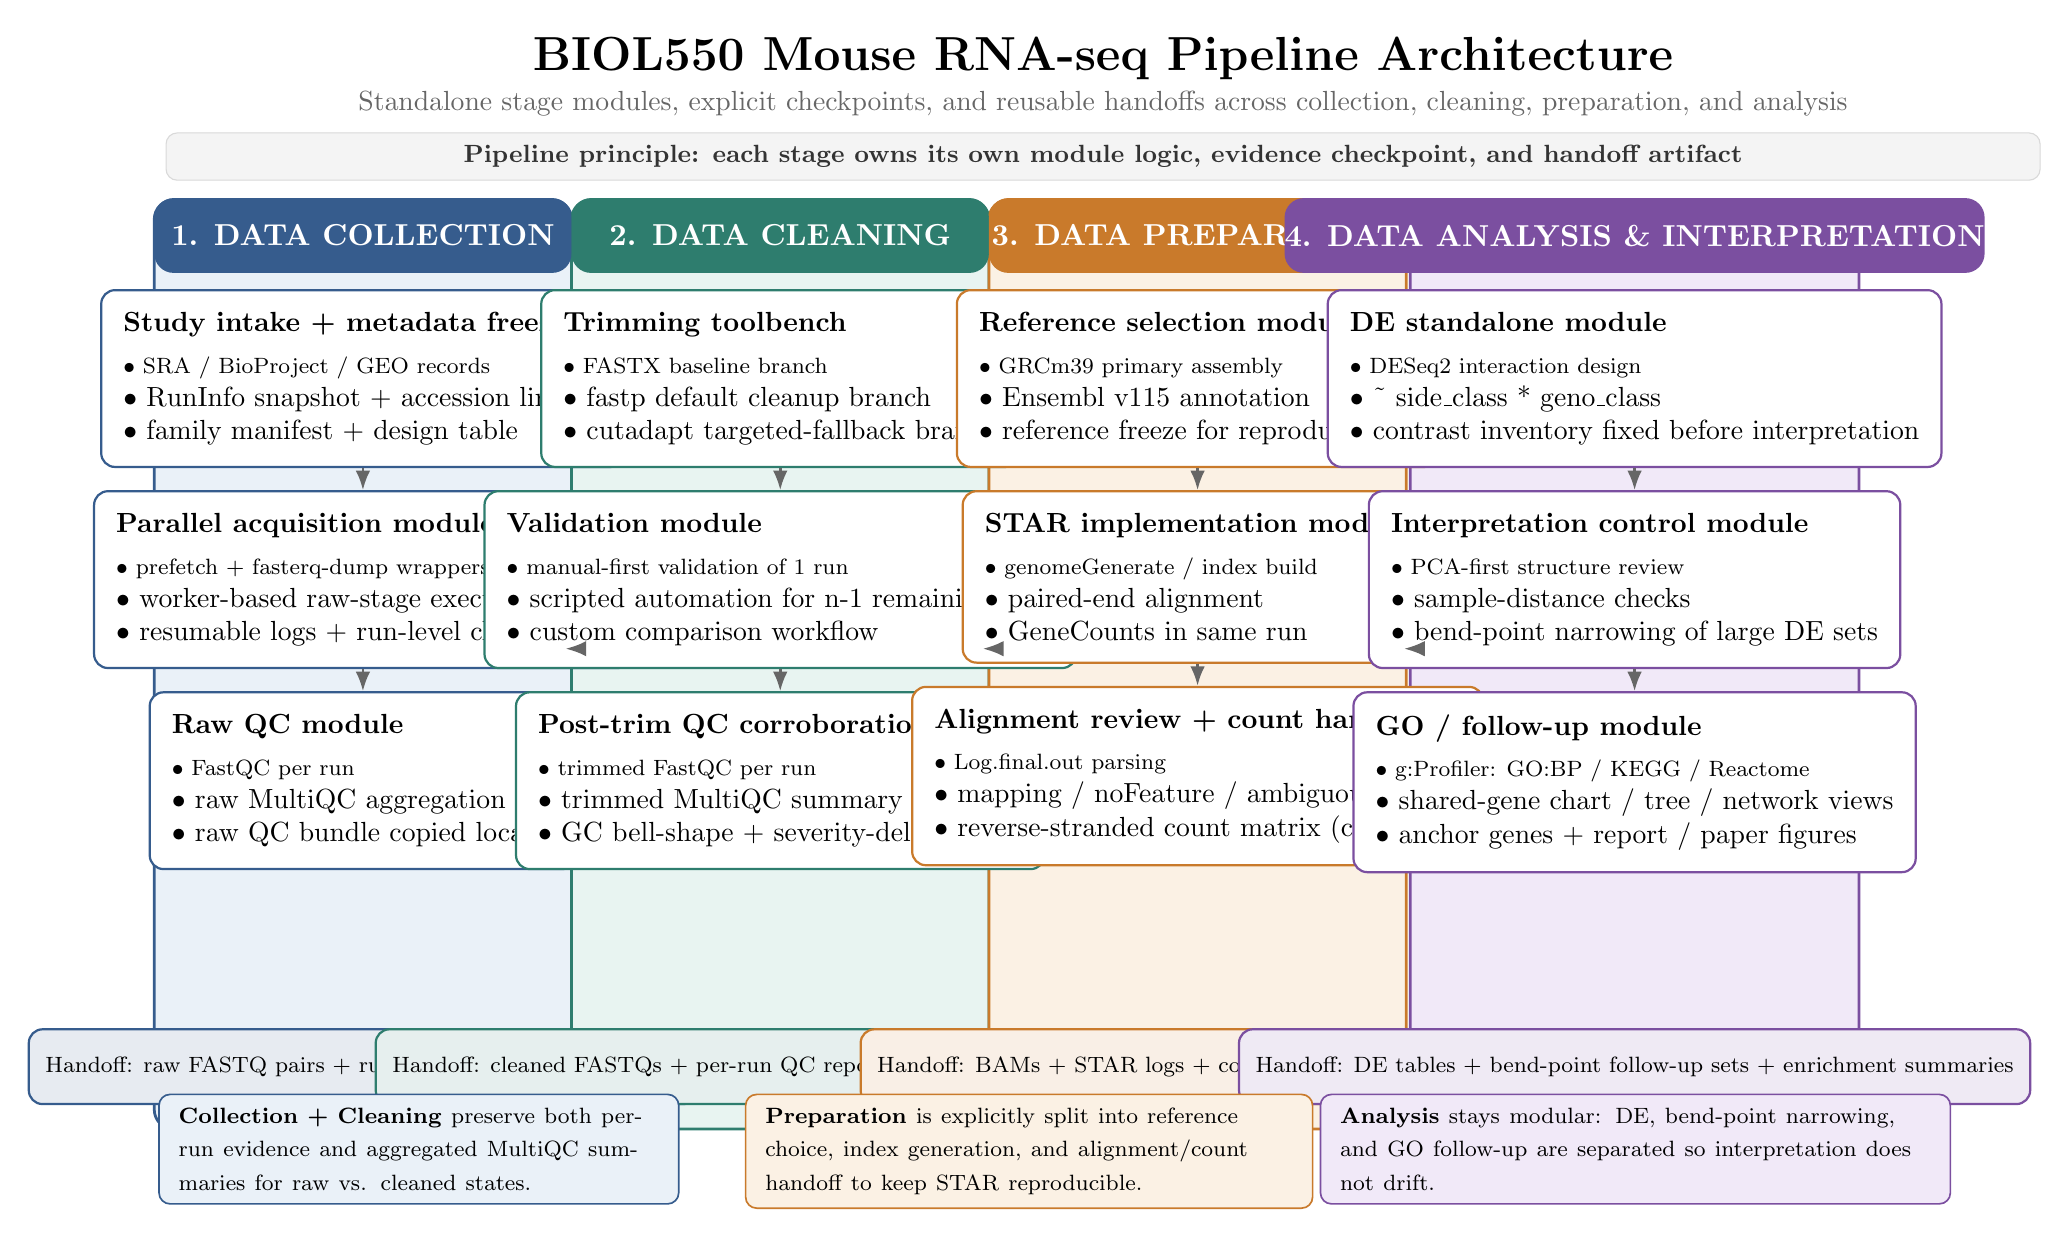
\begin{tikzpicture}[x=1cm,y=1cm]
\node[font=\bfseries\fontsize{17}{18}\selectfont] at (12.25,13.9) {BIOL550 Mouse RNA-seq Pipeline Architecture};
\node[font=\fontsize{9.6}{10.6}\selectfont,text=midgray,align=center] at (12.25,13.32)
{Standalone stage modules, explicit checkpoints, and reusable handoffs across collection, cleaning, preparation, and analysis};
\node[rounded corners=4pt, draw=black!15, fill=lightgray, minimum width=23.8cm, minimum height=0.6cm, font=\bfseries\fontsize{8.7}{9.5}\selectfont, text=black!80, align=center] at (12.25,12.65)
{Pipeline principle: each stage owns its own module logic, evidence checkpoint, and handoff artifact};

\node[stageboxcollect] (S1) at (2.85,6.2) {};
\node[stageboxclean] (S2) at (8.15,6.2) {};
\node[stageboxprep] (S3) at (13.45,6.2) {};
\node[stageboxanalysis] (S4) at (19.0,6.2) {};

\node[stageheadcollect] at ($(S1.north)+(0,-0.47)$) {1. DATA COLLECTION};
\node[stageheadclean] at ($(S2.north)+(0,-0.47)$) {2. DATA CLEANING};
\node[stageheadprep] at ($(S3.north)+(0,-0.47)$) {3. DATA PREPARATION};
\node[stageheadanalysis] at ($(S4.north)+(0,-0.47)$) {4. DATA ANALYSIS \& INTERPRETATION};

\node[modulecollect, anchor=north] (c1) at ($(S1.north)+(0,-1.15)$) {\textbf{Study intake + metadata freeze}\\[3pt]\fontsize{8.1}{9.2}\selectfont $\bullet$ SRA / BioProject / GEO records\\$\bullet$ RunInfo snapshot + accession lineage\\$\bullet$ family manifest + design table};
\node[modulecollect, anchor=north] (c2) at ($(c1.south)+(0,-0.28)$) {\textbf{Parallel acquisition module}\\[3pt]\fontsize{8.1}{9.2}\selectfont $\bullet$ prefetch + fasterq-dump wrappers\\$\bullet$ worker-based raw-stage execution\\$\bullet$ resumable logs + run-level checkpoints};
\node[modulecollect, anchor=north] (c3) at ($(c2.south)+(0,-0.28)$) {\textbf{Raw QC module}\\[3pt]\fontsize{8.1}{9.2}\selectfont $\bullet$ FastQC per run\\$\bullet$ raw MultiQC aggregation\\$\bullet$ raw QC bundle copied locally};
\node[handoffcollect, anchor=south] (ch) at ($(S1.south)+(0,0.32)$) {\fontsize{8.1}{9.2}\selectfont Handoff: raw FASTQ pairs + run manifest + raw QC bundle};

\node[moduleclean, anchor=north] (d1) at ($(S2.north)+(0,-1.15)$) {\textbf{Trimming toolbench}\\[3pt]\fontsize{8.1}{9.2}\selectfont $\bullet$ FASTX baseline branch\\$\bullet$ fastp default cleanup branch\\$\bullet$ cutadapt targeted-fallback branch};
\node[moduleclean, anchor=north] (d2) at ($(d1.south)+(0,-0.28)$) {\textbf{Validation module}\\[3pt]\fontsize{8.1}{9.2}\selectfont $\bullet$ manual-first validation of 1 run\\$\bullet$ scripted automation for n-1 remaining runs\\$\bullet$ custom comparison workflow};
\node[moduleclean, anchor=north] (d3) at ($(d2.south)+(0,-0.28)$) {\textbf{Post-trim QC corroboration}\\[3pt]\fontsize{8.1}{9.2}\selectfont $\bullet$ trimmed FastQC per run\\$\bullet$ trimmed MultiQC summary\\$\bullet$ GC bell-shape + severity-delta review};
\node[handoffclean, anchor=south] (dh) at ($(S2.south)+(0,0.32)$) {\fontsize{8.1}{9.2}\selectfont Handoff: cleaned FASTQs + per-run QC reports + remediation summaries};

\node[moduleprep, anchor=north] (p1) at ($(S3.north)+(0,-1.15)$) {\textbf{Reference selection module}\\[3pt]\fontsize{8.1}{9.2}\selectfont $\bullet$ GRCm39 primary assembly\\$\bullet$ Ensembl v115 annotation\\$\bullet$ reference freeze for reproducibility};
\node[moduleprep, anchor=north] (p2) at ($(p1.south)+(0,-0.28)$) {\textbf{STAR implementation module}\\[3pt]\fontsize{8.1}{9.2}\selectfont $\bullet$ genomeGenerate / index build\\$\bullet$ paired-end alignment\\$\bullet$ GeneCounts in same run};
\node[moduleprep, anchor=north] (p3) at ($(p2.south)+(0,-0.28)$) {\textbf{Alignment review + count handoff}\\[3pt]\fontsize{8.1}{9.2}\selectfont $\bullet$ Log.final.out parsing\\$\bullet$ mapping / noFeature / ambiguous checks\\$\bullet$ reverse-stranded count matrix (col. 4)};
\node[handoffprep, anchor=south] (ph) at ($(S3.south)+(0,0.32)$) {\fontsize{8.1}{9.2}\selectfont Handoff: BAMs + STAR logs + count tables + family matrix};

\node[moduleanalysis, anchor=north] (a1) at ($(S4.north)+(0,-1.15)$) {\textbf{DE standalone module}\\[3pt]\fontsize{8.1}{9.2}\selectfont $\bullet$ DESeq2 interaction design\\$\bullet$ \textasciitilde{} side\_class * geno\_class\\$\bullet$ contrast inventory fixed before interpretation};
\node[moduleanalysis, anchor=north] (a2) at ($(a1.south)+(0,-0.28)$) {\textbf{Interpretation control module}\\[3pt]\fontsize{8.1}{9.2}\selectfont $\bullet$ PCA-first structure review\\$\bullet$ sample-distance checks\\$\bullet$ bend-point narrowing of large DE sets};
\node[moduleanalysis, anchor=north] (a3) at ($(a2.south)+(0,-0.28)$) {\textbf{GO / follow-up module}\\[3pt]\fontsize{8.1}{9.2}\selectfont $\bullet$ g:Profiler: GO:BP / KEGG / Reactome\\$\bullet$ shared-gene chart / tree / network views\\$\bullet$ anchor genes + report / paper figures};
\node[handoffanalysis, anchor=south] (ah) at ($(S4.south)+(0,0.32)$) {\fontsize{8.1}{9.2}\selectfont Handoff: DE tables + bend-point follow-up sets + enrichment summaries};

\draw[downflow] (c1.south) -- (c2.north);
\draw[downflow] (c2.south) -- (c3.north);
\draw[downflow] (d1.south) -- (d2.north);
\draw[downflow] (d2.south) -- (d3.north);
\draw[downflow] (p1.south) -- (p2.north);
\draw[downflow] (p2.south) -- (p3.north);
\draw[downflow] (a1.south) -- (a2.north);
\draw[downflow] (a2.south) -- (a3.north);

\draw[flow] ($(S1.east)+(0.06,0.2)$) -- ($(S2.west)+(-0.06,0.2)$);
\draw[flow] ($(S2.east)+(0.06,0.2)$) -- ($(S3.west)+(-0.06,0.2)$);
\draw[flow] ($(S3.east)+(0.06,0.2)$) -- ($(S4.west)+(-0.06,0.2)$);

\node[notecollect, anchor=north west, minimum width=6.6cm, text width=6.1cm] at (0.25,0.75)
{\fontsize{8.1}{9.2}\selectfont \textbf{Collection + Cleaning} preserve both per-run evidence and aggregated MultiQC summaries for raw vs. cleaned states.};
\node[noteprep, anchor=north west, minimum width=7.2cm, text width=6.7cm] at (7.7,0.75)
{\fontsize{8.1}{9.2}\selectfont \textbf{Preparation} is explicitly split into reference choice, index generation, and alignment/count handoff to keep STAR reproducible.};
\node[noteanalysis, anchor=north west, minimum width=8.0cm, text width=7.5cm] at (15.0,0.75)
{\fontsize{8.1}{9.2}\selectfont \textbf{Analysis} stays modular: DE, bend-point narrowing, and GO follow-up are separated so interpretation does not drift.};

\end{tikzpicture}
\end{document}
